% !TeX root = ../main.tex
\label{sec:proofs}

%We prove the claim that when a classifier recovers the ground truth conditional distribution $\pi(y|x)$, it is also perfectly calibrated. In fact, we only require the weaker assumption that $h(x) = (y^*,p^*)$ if and only if $\pi(y^*|x) = p^*$ where $p^* = \max_{y \in \mathcal{Y}} \pi(y|x)$ and $y^* = \argmax_{y \in \mathcal{Y}} \pi(y|x)$.
%
%{\theorem \label{perfect} A perfect likelihood model achieves perfect calibration in the sense of \autoref{perfect_calibration}.}
%\begin{proof}
%Let $\pi(y|x)$ be the ground truth conditional distribution. The LHS of \autoref{perfect_calibration} becomes
%\begin{align*}
%&\hspace{12pt} \P\left(\yh=Y \sep \ph =p\right) \\
%&=\sum_{y\in \scrY}\P\left(\yh=y ,Y = y\sep \ph =p\right) \\
%&=\sum_{y\in \scrY}\P\left(\yh = y \sep \ph =p\right) \P\left(Y = y \sep \ph =p, \yh = y\right)
%\end{align*}
%We know that $\ph$ and $\yh$ are deterministic functions of $X$ (through our model), so any joint distribution between $\ph,\yh$ and $X$ is nonzero only on points for which $h(X) = (\yh,\ph)$.
%% TODO: Relationship with sufficient statistic?
%Therefore,
%\vspace{-1ex}
%\begin{align*}
%\label{frac_integral}
%&\hspace{12pt} \P\left(Y = y \sep \ph =p, \yh = y\right) \\
%&= \frac{\int_{x\in\scrX} f(X=x,Y=y,\ph=p, \yh = y) dx}{\int_{x\in\scrX} f(X=x,\ph=p, \yh = y) dx} \\
%&= \frac{\int_{x : h(x) = (y,p)} f(X=x,Y=y,\ph=p, \yh = y) dx}{\int_{h(x) = (y,p)} f(X=x,\ph=p, \yh = y) dx} \\
%&= \frac{\int_{x : h(x) = (y,p)}\pi(x)\pi(y|x) dx}{\int_{h(x) = (y,p)}\pi(x) dx}
%\end{align*}
%Now consider the true likelihood $\pi(y|x)$. Because we have a perfect likelihood model, $\pi(y|x) = \hat{\pi}(y|x)$. But inside the integral, $\hat{\pi}(y|x) = p$ since $f(x) = (y,p)$, so $\pi(y|x)=p$, and (\ref{frac_integral}) reduces to $p\frac{\int_{f(x) = (y,p)}\pi(x) dx}
%{\int_{f(x) = (y,p)}\pi(x) dx} = p$. Plugging this back into gives us $\P(\yh=Y\sep \ph =p) = p$,
%%because $\sum_{y\in \scrY}\P(\yh = y| \ph =p) = 1$,
%which is the desired result. With $\ph \in (p-\delta,p+\delta)$, we instead get $\pi(y|x)\in (p-\delta,p+\delta)$, and eventually $\P(\yh=Y\sep \ph =p)\in (p-\delta,p+\delta)$. This gives the $(\delta,\delta)$ guarantee. \end{proof}
%% TODO: This proof currectly doesn't work since the probability with \ph = p can be 0, and cannot be placed in the denominator. Need a more "mathematical" proof (maybe in the Appendix).

%This motivates the next empirical definition with respect to a finite set of samples.
%{\definition($\epsilon,\delta$-calibration, empirical)
% A classifer $f$ is $\epsilon,\delta$-calibrated in the empirical sense if $~\forall p\in(0,1)$,
%\begin{equation}
%\label{frac_math}
%\bigg| \frac{\sum_{i=1}^{n}\ind_{(p-\delta,p+\delta)}(\hat{p}_i)\ind_{y_i}(\hat{y}_i)}
%{\sum_{i=1}^{n}\ind_{(p-\delta,p+\delta)}(\hat{p}_i)}
%- p \bigg| < \epsilon
%\end{equation}
%}
%Note that the fraction in (\ref{frac_math}) is simply a more rigorous statement of that in (\ref{frac_text}).

\label{sup:proof}
Here we derive the temperature scaling model using the entropy maximization principle with an appropriate balanced equation.
%
{\claim \label{max-entropy} Given $n$ samples' logit vectors $\zb_1, \ldots, \zb_n$ and class labels $y_1, \ldots, y_n$, temperature scaling is the unique solution $q$ to the following entropy maximization problem:
\begin{align*}
\max_{q} \hspace{8pt} & -\sum_{i=1}^n \sum_{k=1}^K q(\zb_i)^{(k)} \log q(\zb_i)^{(k)} \\
\text{subject to} \hspace{10pt} & q(\zb_i)^{(k)} \geq 0 \hspace{30pt} \forall i, k \\
                                & \sum_{k=1}^K q(\zb_i)^{(k)} = 1 \hspace{12pt} \forall i \\
																& \sum_{i=1}^n z_i^{(y_i)} = \sum_{i=1}^n \sum_{k=1}^K z_i^{(k)} q(\zb_i)^{(k)}.
\end{align*}}
%
The first two constraint ensure that $q$ is a probability distribution, while the last constraint limits the scope of distributions. Intuitively, the constraint specifies that the average true class logit is equal to the average weighted logit.
%
\begin{proof}
We solve this constrained optimization problem using the Lagrangian. We first ignore the constraint $q(\zb_i)^{(k)}$ and later show that the solution satisfies this condition. Let $\lambda,\beta_1,\ldots,\beta_n \in \mathbb{R}$ be the Lagrangian multipliers and define
\begin{align*}
L = &-\sum_{i=1}^n \sum_{k=1}^K q(\zb_i)^{(k)} \log q(\zb_i)^{(k)} \\
    & + \lambda \sum_{i=1}^n \left[ \sum_{k=1}^K z_i^{(k)} q(\zb_i)^{(k)} - z_i^{(y_i)} \right] \\
	  & + \sum_{i=1}^n \beta_i \sum_{k=1}^K (q(\zb_i)^{(k)} - 1).
\end{align*}
Taking the derivative with respect to $q(\zb_i)^{(k)}$ gives $$\frac{\partial}{\partial q(\zb_i)^{(k)}} L = -nK - \log q(\zb_i)^{(k)} + \lambda z_i^{(k)} + \beta_i.$$
Setting the gradient of the Lagrangian $L$ to 0 and rearranging gives $$q(\zb_i)^{(k)} = e^{\lambda z_i^{(k)} + \beta_i - nK}.$$
Since $\sum_{k=1}^K q(\zb_i)^{(k)} = 1$ for all $i$, we must have $$q(\zb_i)^{(k)} = \frac{e^{\lambda z_i^{(k)}}}{\sum_{j=1}^K e^{\lambda z_i^{(j)}}},$$
which recovers the temperature scaling model by setting $T = \frac{1}{\lambda}$. 
\end{proof}

\autoref{figure.entropy} visualizes Claim \autoref{max-entropy}.
We see that, as training continues, the model begins to overfit with respect to NLL (red line).
This results in a low-entropy softmax distribution over classes (blue line), which explains the model's overconfidence. Temperature scaling not only lowers the NLL but also raises the entropy of the distribution (green line).

\begin{figure*}[h!]
	\centering
	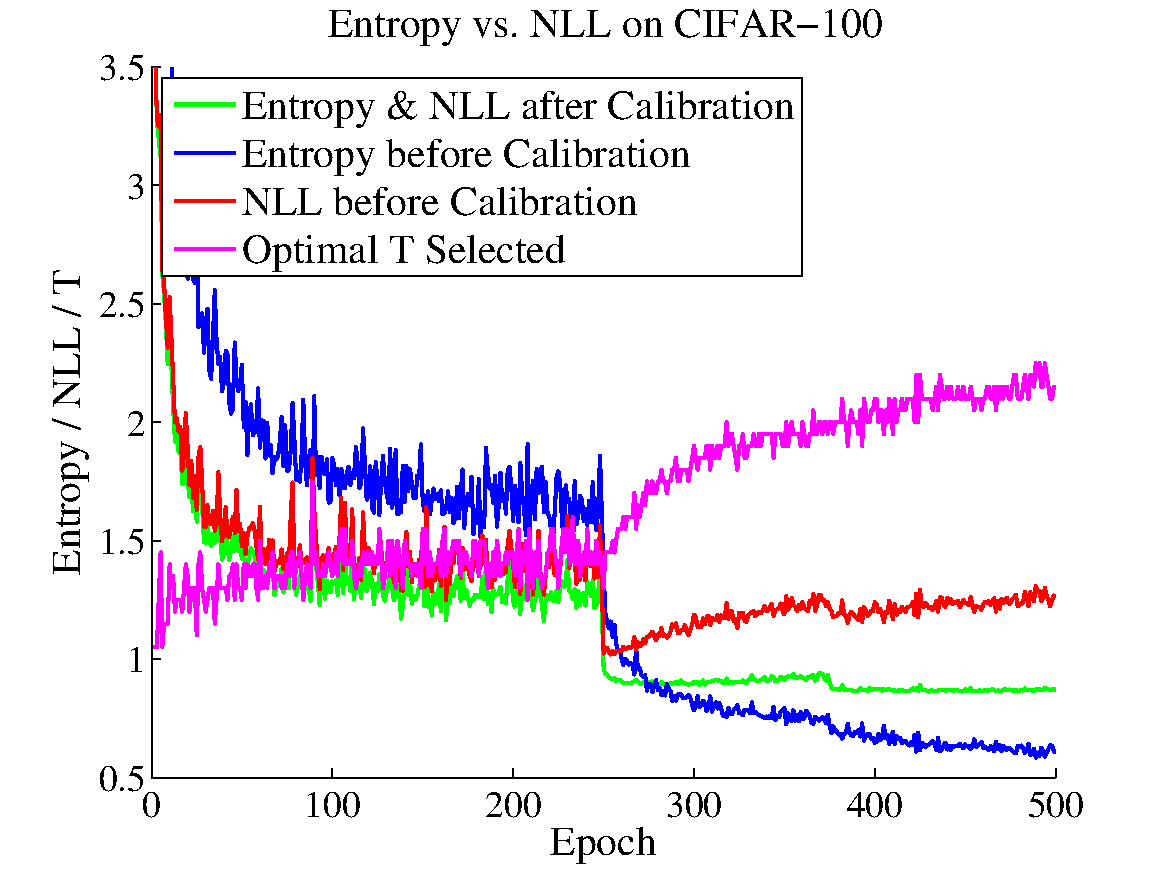
\includegraphics[width=1.5\columnwidth]{fig/entropy-cifar100.pdf}
	\caption{Entropy and NLL for CIFAR-100 before and after calibration. The optimal $T$ selected by temperature scaling rises throughout optimization, as the pre-calibration entropy decreases steadily.
	The post-calibration entropy and NLL on the validation set coincide 
	(which can be derived from the gradient optimality condition of $T$). }
	\label{figure.entropy}
\end{figure*}



%{\theorem
%\label{l2equiv}
%Suppose $f_\wb$ is a feedforward neural network of depth $L$ with ReLU activation units, and possibly max / average pooling. That is, for $l=1...L$,
%$$\xb^{(l)} = \text{pool}\left(\text{ReLU}\left( \xb^{(l-1)}\wb^{(l)}\right) \right)$$
%where $\xb^{(0)}$ is the input matrix, and $\xb^{(l)}$ is the output of the $l^{th}$ layer.
%Then the following three procedures produce equivalent models:
%\begin{enumerate}[label={\alph*)},itemsep=0.5pt,topsep=0pt]
%\item optimizing a weight decay loss function $\frac{1}{2}\lambda\|\wb\|^2_2$ for one iteration of gradient descent, where $\lambda\in(0,1)$ is a (usually very small) tunable hyperparameter.
%\item weight shrinkage by a factor of $(1-\lambda)$.
%\item setting $T=(1-\lambda)^{-L}$ in (\ref{temp}).
%\end{enumerate}
%}
%\begin{proof}
%The equivalence between a) and b) is widely known, that is, because $\frac{\partial}{\partial \wb} \frac{1}{2}\lambda\|\wb\|^2_2 = \lambda\wb$, we have that $\wb - \frac{\partial}{\partial \wb} \frac{1}{2}\lambda\|\wb\|^2_2 = (1-\lambda)\wb$. To get the equivalence between b) and c), we note that $1-\lambda$ is also in $(0,1)$, so
%$$\text{ReLU}\left( \xb^{(l-1)}(1-\lambda)\wb^{(l)}\right) = (1-\lambda)\text{ReLU}\left( \xb^{(l-1)}\wb^{(l)}\right)$$
%So the $(1-\lambda)$ factor propagates through each nonlinearity, and
%the same applies for max / average pooling. Altogether, each of the $L$ layers propagates a factor of $(1-\lambda)$, and by the end of the chain, we have
%$$\xb^{(L)} = (1-\lambda)^L\text{pool}\left(\text{ReLU}\left( \xb^{(L-1)}\wb^{(L)}\right) \right)$$
%But $\xb^{(L)}$ contains exactly the logits, that is, $\xb^{(L)}_{k} = z_k$. By making the temperature the inverse of $(1-\lambda)^L$, we recover the multiplicative factor and this proves the theorem.
%\end{proof}
%Note that we can incorporate the bias terms into $\wb^{(l)}$ (by padding $\xb^{(l)}$ with 1s at the top). This theorem practically covers all the modern network architectures, including CNNs and those with Batch Normalization~\cite{ioffe2015batch}.